\documentclass[12pt, fleqn, xcolor=x11names, xcolor=table, aspectratio=169]{beamer}
\beamertemplatenavigationsymbolsempty
% \usefonttheme[onlymath]{serif}

\usecolortheme{beaver}
\setbeamertemplate{blocks}[rounded=true, shadow=true]
\setbeamertemplate{footline}[page number]
\setbeamercolor{itemize item}{fg=red}
\setbeamercolor{enumerate item}{fg=red}
% \usepackage{jmlda}

%
\usepackage[T2A]{fontenc}
\usepackage[utf8]{inputenc}
\usepackage[english,russian]{babel}
\usepackage{amsmath, amsfonts,amssymb,mathrsfs}

\usepackage{multirow}
\usepackage{multicol}% many columns in slide
\usepackage{hyperref}% urls
\usepackage{hhline}%tables
\usepackage[export]{adjustbox}

\usepackage{xcolor, color, colortbl}
\usepackage[table]{xcolor}
\definecolor{aquamarine}{rgb}{0.5, 1.0, 0.83}
\definecolor{blue-green}{rgb}{0.0, 0.87, 0.87}
\definecolor{magicmint}{rgb}{0.67, 0.94, 0.82}
\usepackage{tabularx}
\newcommand\setrow[1]{\gdef\rowmac{#1}#1\ignorespaces}
\renewcommand{\footnotesize}{\fontsize{7pt}{9pt}\selectfont}

% \expandafter\show\the\font
%----------------------------------------------------------------------------------------------------------
\title{Оптимизация критерия, заданного нейросетевой моделью, в задаче детоксификации текста}
\author[А.\,A.~Пилькевич]{А.\,A.~Пилькевич}
\institute{Московский физико-технический институт}
\date{\footnotesize
% \par\smallskip\emph{Курс:} Автоматизация научных исследований\par (практика, В.\,В.~Стрижов)/Группа 874
\par\smallskip\emph{Научный руководитель:} д.ф.-м.н. К.\,В.~Воронцов,  д.ф.-м.н. В.\,В.~Стрижов
\par\smallskip\emph{Консультант:} А.\,С.~Попов
\par\bigskip\small 2022}
%----------------------------------------------------------------------------------------------------------
\def\vec#1{\mathchoice{\mbox{\boldmath$\displaystyle#1$}}
{\mbox{\boldmath$\textstyle#1$}} {\mbox{\boldmath$\scriptstyle#1$}} {\mbox{\boldmath$\scriptscriptstyle#1$}}}
\begin{document}
%----------------------------------------------------------------------------------------------------------
\begin{frame}
\thispagestyle{empty}
\maketitle
\end{frame}

%-----------------------------------------------------------------------------------------------------
\begin{frame}{Детоксификация предложений}

\begin{alertblock}{Задача}
Стилизация токсичных (частично обсценных) входных предложений к нейтральному варианту. Для оценки качества используется нейросетевая модель степени токсичности.
\end{alertblock}

\begin{alertblock}{Проблема}

Модель невозможно использовать в качестве функции потерь из-за различия входных данных, так как теряется её дифференцируемость по параметрам. 
\end{alertblock}

\begin{alertblock}{Решение}
Предлагается <<адаптировать>> оценочную модель, чтобы она принимала распределения вероятностей токенов, выданных детоксификатором. 
\end{alertblock}

\end{frame}
%-----------------------------------------------------------------------------------------------------
\begin{frame}{Данные и оценка качества детоксификации}
Дано множество пар  $(s_{t}, s_{d})$:
\begin{table}[ht]
\centering
 \begin{tabular}{|l|l|} 
 \hline 
 $s_{t}$~--- токсичное предложение & $s_{d}$~---~нейтральная версия \\
 \hline
 \textit{<<Её муженька козла на кол надо посадить.>>} & \textit{<<Её мужа нужно наказать.>>} \\
 \textit{<<Это твари а не люди.>>} & \textit{<<Это плохие люди.>>} \\
 \hline
 \end{tabular}
\end{table}


\vfill

\textbf{Требуется:} по токсичному предложению построить нейтральное.

\vfill

\textbf{Качество стилизация текста оценивается:} 
\begin{itemize}
    \item точностью соответствия заданному стилю,
    \item качеством сохранения смысла после перефраза.
\end{itemize}

\end{frame}

%-----------------------------------------------------------------------------------------------------
\begin{frame}{Автоматическая оценка качества детоксификации}

\textbf{Style Transfer Accuracy (STA)} --- Conversational RuBERT\footnote{\url{https://huggingface.co/DeepPavlov/rubert-base-cased-conversational}}. 
Модель классификации, предсказывающая вероятность токсичности предложения.
Отвечает за стилизацию текста. 

\vfill

\textbf{chrF} --- F-score на основе символьных $n$-грамм\footnote{Popović M. \textit{chrF: character n-gram F-score for automatic MT evaluation} – 2015.}. 
Отвечает за сохранение смысла:
\begin{gather*}
    \text{chrF}_\beta = (1 + \beta^2) \frac{\text{chrP} \cdot \text{chrR}}{\beta^2 \text{chrP} + \text{chrR}},
\end{gather*}

\begin{itemize}
    \item chrP --- доля символьных $n$-грамм из предлагаемого предложения, которые имеются в оригинальном. 
    
    \item chrR --- доля символьных $n$-грамм из оригинального предложения, которые представлены в предлагаемом: 

\end{itemize}

\end{frame}

%----------------------------------------------------------------------------------------------------------


\begin{frame}{Детоксификация как машинный перевод}

Поставим задачу детоксификации как задачу машинного перевода (seq-to-seq) для пар предложений $(t, d)$:
\begin{itemize}
    \item $t = \tau_f(s_t)$, $d = \tau_f(s_d)$,
    \item $\tau_f$ --- токенизатор, переводящий текст в последовательность BPE-токенов из словаря $V_f$.
\end{itemize}

\vfill

Архитектура задаётся моделью кодировщик-декодировщик $f_{\theta}$ на основе предобученного ruT5-base\footnote{Raffel C. et al. \textit{Exploring the limits of transfer learning with a unified text-to-text transformer} – 2019.}. 
\begin{gather*}
    \mathcal{L}_{\text{CE}} = -\sum_{i=1}^{n} \log f_\theta(d_{i} | d_{<i}, t) \longrightarrow \min_{\theta}, \\
    f_{\theta}(* | d_{<i}, t) \in [0, 1]^{|V_f|} \text{~--- распределение вероятностей}.
\end{gather*}
\end{frame}


%----------------------------------------------------------------------------------------------------------

\begin{frame}{Детоксификация как задача стилизации}

% Предлагается использовать STA-модель 
% $g_{\text{toxic}}: \left(V_g\right)^{\times n} \to [0, 1]$ 
% в качестве функции потерь 
% $\mathcal{L}_{\text{TP}} = g_{\text{toxic}}\bigl(\tau_{g}(s) \bigr)$, 
% где $\tau_{g}: \text{текст} \to \left(V_g\right)^{\times m}$~--- токенизатор STA-модели и $V_g$~--- её словарь. 

% \vfill

% Но требуется получить 
% $s_{\text{detox}} = \{\arg\max_{d_i} f_{\theta}(d_{i} | d_{<i}, t)\}_{i=1}^{n}$~--- сырой текст, чтобы посчитать 
% $\mathcal{L}_{\text{TP}} =  g_{\text{toxic}}\bigl(\tau_{g}(s_{\text{detox}}) \bigr)$

% \vfill

% $\mathcal{L}_{\text{TP}}$ не дифференцируема по параметрам детоксификатора $
% \theta$, так как \textbf{нет инъективного отображения между токенами различных токенайзеров}. 
% \begin{gather*}
%     \text{ты слишком токсичный} \longrightarrow 
%     \begin{cases} 
%         [\text{ты},\ \text{слишком},\ \text{токс},\ \text{ич},\ \text{ный}],\ &\tau_{f}, \\
%         [\text{ты},\ \text{\#UNK},\ \text{токсичн},\ \text{ый}],\ &\tau_{g}.
%     \end{cases}
% \end{gather*}


Предлагается использовать STA-модель 
$g_{\text{toxic}}$ в качестве функции потерь:
\begin{gather*}
    \mathcal{L}_{\text{TP}} = g_{\text{toxic}}\bigl(\tau_{g}(s_{detox}) \bigr) \to \min_\theta.
\end{gather*}

\begin{itemize}
    \item $\tau_{g}$~--- токенизатор, переводящий текст в последовательность BPE-токенов из словаря $V_g$,
    \item $s_{detox}$~--- результат работы детоксификатора:
    \[
    s_{\text{detox}} = \{\arg\max_{d_i} f_{\theta}(d_{i} | d_{<i}, t)\}_{i=1}^{n}.
    \]
    
\end{itemize}

$\mathcal{L}_{\text{TP}}$ не дифференцируема по параметрам детоксификатора $
\theta$, в силу недифференцируемости функции $\tau_g$ и $\arg \max$!

\begin{gather*}
    \textit{ты слишком токсичный} \longrightarrow
    \begin{cases} 
        [\textit{ты},\ \textit{слишком},\ \textit{токс},\ \textit{ич},\ \textit{ный}] &\text{ от } \tau_{f}\\
        [\textit{ты},\ \textit{\#UNK},\ \textit{токсичн},\ \textit{ый}] &\text{ от } \tau_{g}.
    \end{cases}
\end{gather*}

\end{frame}

%----------------------------------------------------------------------------------------------------------

\begin{frame}{Адаптер~--- аппроксимация векторного представления}

\begin{columns}[c]
\column{.63\textwidth}

Хотим при фиксированных параметрах STA-модели $g_{\text{toxic}}$ выполнения:
\begin{gather*}
    g_{\text{toxic}}\bigl(\tau_{g}(s_d) \bigr) \approx 
    g^{*}_{\text{toxic}} \bigl(f_{\theta} \bigl(\tau_{f}(s_t)\bigr) \bigr).
\end{gather*}

\vfill

$g^{*}_{\text{toxic}}$~--- STA-модель, в которой заменили входной эмбеддинг слой  \textit{адаптером} $A \in \mathbb{R}^{|V_f| \times e}$,
где $e$~--- размерность векторного представления токенов.

\vfill

Причём $g^{*}_{\text{toxic}}$ принимает $f_{\theta}(*) \in [0, 1]^{n \times |V_f|}$~--- <<зашумлённые one-hot вектора>>.

\column{.3\textwidth}
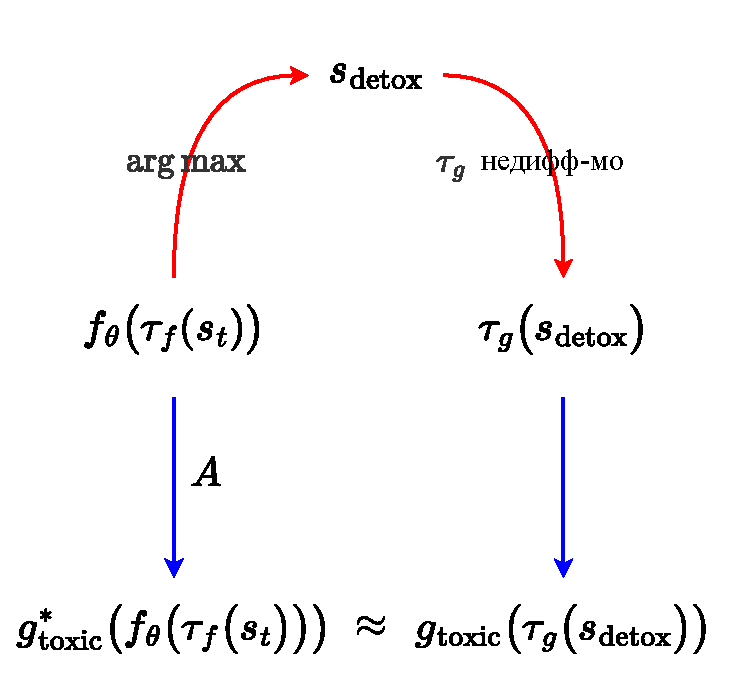
\includegraphics[width=1.2\textwidth, left]{images/non_diff_loss.pdf}
\end{columns} 
\end{frame}

%----------------------------------------------------------------------------------------------------------

\begin{frame}{Обучение адаптера}
\begin{columns}[c]
\column{.63\textwidth}

\textbf{Выход STA-модели}:

$P_{\text{toxic}} =g_{\text{toxic}}\bigl(\tau_{g}(s_d) \bigr)$~--- вероятность токсичности предложения $s_d$,

$P^{*}_{\text{toxic}} = g^{*}_{\text{toxic}} \bigl(f_{\theta} \bigl(\tau_{f}(s_t)\bigr) \bigr)$~--- вероятность токсичности с использованием адаптера для $s_t$. 

 

\vfill

\textbf{Функция потерь адаптера}: 
$D_\text{KL}(P_{\text{toxic}} \parallel P^{*}_{\text{toxic}}) \longrightarrow \min_{A}.$

\vfill

\begin{alertblock}{Алгоритм обучения $A$}
\begin{enumerate}
    \item Обучается детоксификатор $f_{\theta}$ на задаче seq-to-seq.
    \item Обучается адаптер $A$ при фиксированных параметрах $f_{\theta}$ и STA-модели.
\end{enumerate}
\end{alertblock}

\column{.3\textwidth}
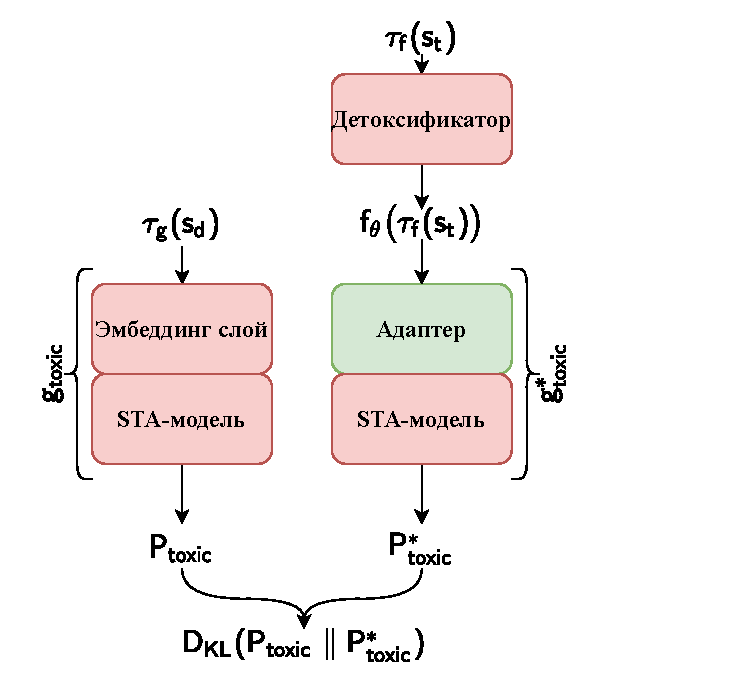
\includegraphics[width=1.5\textwidth, left]{images/pres_adapter_train2.pdf}
\end{columns} 
\end{frame}

%----------------------------------------------------------------------------------------------------------

\begin{frame}{Дообучение детоксификатора}
При дообучении детоксификатора $f_{\theta}$ используется схожая идея с обучением порождающих моделей\footnote{Goodfellow I. et al. \textit{Generative adversarial nets} – 2014.}.

\vfill

Пусть $\text{CE, TP}$~--- значение кросс-энтропии $\mathcal{L}_{\text{CE}}$ и выход STA-модели $\mathcal{L}_{\text{TP}}$.

$F(*, *)$~--- произвольная функция для агрегации функционалов, $F: \mathbb{R}^2 \to \mathbb{R}$.

\vfill

\begin{alertblock}{Алгоритм дообучения $f_{\theta}$}
\begin{enumerate}
    \item $N$ батчей обучается $f_{\theta}$ на $F(\text{CE, TP})$, при фиксированных параметрах $A$. 
    \item $M$ батчей обучается $A$ на $D_\text{KL}$, при фиксированных параметрах $f_{\theta}$.
\end{enumerate}
\end{alertblock}
\end{frame}

%----------------------------------------------------------------------------------------------------------

\begin{frame}{Эксперименты по детоксификации}

Обучающая выборка: $11136$ пар $\left(s_t, s_d \right)$, $10\%$ использовались для валидации во время обучения.
Тестовой выборка: $800$ предложений.

\vfill

Результаты экспериментов в различных конфигурациях обучения:
\begin{table}[ht]
\centering
 \begin{tabular}{|l l|c c c|} 
 \hline
 Подход & F(\text{CE, TP}) & STA & chrF1 & STA*chrF1 \\ [0.5ex] 
 \hline
 seq-to-seq & CE & 0.739 & 0.578 & 0.427 \\ 
  GAN style & $\text{CE} \cdot \text{TP}$  & 0.754 & 0.574 & 0.439 \\
 \rowcolor{magicmint} GAN style & $\text{CE} + w_2 \text{TP}$ & 0.813 & 0.569 & 0.462 \\
 seq-to-seq & TP & 0.998 & 0.119 & 0.119 \\ 
 \hline
 \end{tabular}
\end{table}


\vfill
Наилучшее качество показывает линейное взвешивание функций потерь, что позволяет задать приоритет для оптимизируемого функционала.

\end{frame}

%----------------------------------------------------------------------------------------------------------

\begin{frame}{Проверенные подходы обучения}

Проверка статистической значимости, когда на одном батче сперва оптимизировался детоксификатор, затем адаптер:
\begin{table}[ht]
\centering
 \begin{tabular}{|l l|c c c|} 
 \hline
 Подход & F(\text{CE, TP}) & STA & chrF1 & STA*chrF1 \\ [0.5ex] 
 \hline
 seq-to-seq & CE & $0.744 \pm 0.010$ & $0.575 \pm 0.002$ & $0.430 \pm 0.042$ \\ 
 Same batch & $\text{CE} \cdot \text{TP}$ & $0.776 \pm 0.015$ & $0.569 \pm 0.004$ & $0.442 \pm 0.006$ \\
 Same batch & $\text{CE} + w_2 \text{TP}$ & $0.774 \pm 0.011$ & $0.561 \pm 0.012$ & $0.435 \pm 0.013$ \\

  \hline
 \end{tabular}
\end{table}

Эксперимент с одновременным обучением детоксификатора и адаптера на одинаковую функцию потерь:
\begin{table}[ht]
\centering
 \begin{tabular}{|l|c c c|} 
 \hline
 Подход & STA & chrF1 & STA*chrF1 \\ [0.5ex] 
 \hline
 seq-to-seq CE & 0.742 & 0.577 & 0.428  \\ 
 Adapter on embs & 0.639 & 0.544 & 0.348 \\
 Adapter on logits & 0.708 & 0.569 & 0.403 \\

  \hline
 \end{tabular}
\end{table}

\end{frame}


%----------------------------------------------------------------------------------------------------------
\begin{frame}{Выносится на защиту}

\begin{enumerate}
    \item Предложен алгоритм использования нейросетевой модели в качестве функции потерь в условиях отсутствия дифференцируемость, так как нет отображения между токенами различных токенайзеров.
    
    \item Продемонстрирована работоспособность и эффективность предложенного метода. 
    
    \item Подобраны оптимальные параметры совместного обучения детоксификатора и адаптера. 
    
    \item Реализован и опубликован код для воспроизведения экспериментов из представленной работы\footnote{\url{https://github.com/Intelligent-Systems-Phystech/Pilkevich-BS-Thesis}}.
    
\end{enumerate}

\end{frame}

%----------------------------------------------------------------------------------------------------------
\end{document} 
